\begin{chapter}{Physical Model\label{chap:physical}}

Section \ref{sec:intro.prob_def} describes the basic activation
process and shows a sample activation tree in figure
\ref{fig:intro.basic_tree}.  Figure \ref{fig:physical.basic_tree}
shows the same tree with annotations to define the nomenclature to be
used in this chapter and others.

\begin{floatingfigure}{0.55\columnwidth}
  \begin{center}
    \epsfig{file=eps/annotated_basic_tree.eps,width=0.5\columnwidth}
    \caption{Annotated sample activation tree showing loops and
      cross-links.}\label{fig:physical.basic_tree}
  \end{center}
\end{floatingfigure}

A tree is constructed of \textsl{nodes}, each representing a single
isotope, and \linebreak \textsl{branches}, each representing a reaction path
between the \textsl{parent} isotope and \textsl{daughter} isotope for
that reaction.  The top isotope in the tree will be called the
\textsl{root} and each succeeding generation of reaction products will
be referred to as a \textsl{rank}, giving a measure of the depth of
the tree.  Each isotope has a production rate, $P_{ij}$ (the root has
no production rate), dependent on the reaction path by which it was
produced, and a unique total destruction rate, $d_i$.  For decay
reactions, this production rate is dependent only on the parent's
nuclear data (specifically, the half-life) and not on the neutron
flux.  For transmutation reactions, it is a function of the parent's
nuclear data and the spectral distribution of the flux.  The
destruction rate may be made of a combination of transmutation data,
and thus the neutron flux, and decay data, depending on the parent
isotope.  The raw data used to form these production rates are read
from large data libraries, either as decay rate/branching ratio data
from decay libraries or as transmutation cross-sections from
transmutation libraries.  While the methods used to measure, evaluate
and compile such data\cite{EAF,FENDL2} will not be discussed here, it
is important to note that seemingly small changes in these data can
lead to observable differences in the results of an activation
calculation.

It is possible for one nucleus to undergo a series of reactions, being
converted from one isotope to another and so on and eventually back to
the original isotope.  Loops such as this are of specific importance
when modeling this physical problem.  The nature of such loops is
somewhat random; they can begin at any rank in the tree and can
undergo any number of reactions before closing the loop.  If the
\textsl{order} of a loop is defined here as the number of isotopes
between two occurrences of the same isotope in a loop, then the order
can range from 1 to greater than 10.  Loops are only physically
possible during irradiation.  During periods of pure decay, loops are
physically disallowed for the simple reason that nuclear decay is a
transition to a lower energy state.  This can only be reversed by the
introduction of an energy source, provided by the bombarding neutrons
during irradiation.  One example of a loop is
\begin{equation*}
  ^{28}\mathrm{Si} \stackrel{(n,p)}{\longrightarrow} \ ^{28}\mathrm{Al}
  \stackrel{\beta^-}{\longrightarrow} \ ^{28}\mathrm{Si},
\end{equation*}
in which $^{28}$Si is transmuted by a neutron reaction with the
emission of a proton to $^{28}$Al.  $^{28}$Al, in turn, decays back to
$^{28}$Si through the emission of a $\beta^-$ particle.  There are
many other variations of loops, involving different nuclear reactions
and with more than two isotopes involved in the loop.
    
A related but less important phenomenon is that of
\textsl{cross-linking} of subtrees.  This is caused when two different
isotopes, which could each be at any rank, both undergo reactions to
the same isotope.  Between loops and cross-links, the tree can become
quite tangled, departing from the classical tree structure known and
studied in computer science.

Since most isotopes will undergo nuclear reactions, as soon as they
are created by either transmutation or decay, there is a finite chance
of them being transmuted to other isotopes.  As a result, an
activation tree can, in theory, grow to become a large connected graph
including all the isotopes for which data exists, with many
cross-links and loops of various orders.  If many reactions are
required to reach a certain isotope from the root isotope, however,
their production levels will be insignificant.  For the purpose of a
practical numerical solution, therefore, it is necessary to truncate
the tree based on some reasonable criteria.

The methods for modeling activation trees, including loop handling and
tree truncation, can have a significant impact both on the type of
mathematical technique employed to generate a solution, and on the
accuracy of the results.  Section \ref{sec:physical.chains} addresses
these issues and others in the creation of activation trees.

Current designs for fusion power reactors of all types often include
the necessity for pulses, from the short frequent pulses of an
inertial confinement system to the long infrequent pulses of a
magnetic confinement system.  Other neutron-producing systems, such as
experimental fusion reactors or accelerator-based neutron sources, may
have more complicated irradiation histories, with varying pulsing
frequencies, pulsing hierarchies, maintenance periods, etc.
Furthermore, with changing conditions the flux spectrum and/or
magnitude may differ from one part of the history to another.  This
pulsing creates an important effect\cite{Pulsar,spangler,spanglerMS}
since between each pulse, the radioactive isotopes which have been
created are able to decay while the stable isotopes remain unchanged.
This changes the distribution of isotopes, having important
implications on the reactions during the subsequent pulses.  Section
\ref{sec:physical.pulsing} will describe the approximations and
assumptions used in modeling this aspect of the physical model.

Although activation calculations have traditionally been used to find
all the activation products of a given material composition exposed to
a given neutron flux history, this mode is not suited to the task of
determining the concentrations of specific trace activation products.
If certain isotopes are produced in very small quantities, the
accurate determination of their concentration requires that the
activation trees be allowed to grow to large sizes, and much
computational effort will be wasted calculating the concentrations of
uninteresting isotopes.  Using many of the same modeling methods
described in this chapter, small modifications can lead to a
\textsl{reverse} activation calculation mode, whereby the
concentrations of certain target isotopes can be calculated from the
initial mixtures without calculating the concentrations of too many
non-target isotopes.  Section \ref{sec:physical.reverse} describes the
adaptations necessary for such a reverse calculation.

The last section of this chapter addresses some of the software design
and implementation issues related to the various modeling methods
discussed for the physical problem, including data structures,
computational efficiency and optimum memory usage.

\begin{section}{Activation Tree Modeling\label{sec:physical.chains}}
  
  As mentioned above, the theoretical activation tree can become a
  large connected graph including every isotope for which data exists.
  This could, in principle, be converted into a large matrix of
  production and destruction rates, and solved directly for all the
  initial isotopes at a given point in space.  This is not practical,
  however, both due to the size of the matrix and the mathematical
  methods available for solving such a matrix.  For a typical fusion
  activation library, the matrix would be roughly $2000 \times 2000$,
  sparsely filled (only about 1 or 2\%) and would exhibit little
  pattern (\textsl{i.e.} banded or triangular matrices).  By
  introducing a variety of concepts, this problem can be reduced to a
  finite number of tractable sub-problems.  
  
  There are two primary issues related to the modeling of activation
  trees: loop handling and tree truncation.
  
  \begin{subsection}{Tree Straightening and Loop Handling\label{sec:physical.chains.loops}}
    
    \begin{floatingfigure}{0.55\columnwidth}
      \begin{center}
        \epsfig{file=eps/straight_tree.eps,width=0.5\columnwidth} 
        \caption{Fully straightened and unlinked reaction
          tree.}\label{fig:physical.straight_tree}
      \end{center}
    \end{floatingfigure}
    
    \noindent One alternative for loop handling is to explicitly model them in
    the mathematical representation of the physical problem.  In the
    rate equation for node $i$, there is a production term from some
    node $j>i$ and in the matrix formulation shown in equation
    \ref{eqn:intro.basic_ode}, the transfer matrix, \mat{A}, has terms
    above the diagonal.  While time-step based ODE solvers can be used
    with this method\cite{FISPACT}, the non-triangular nature of this
    matrix limits the matrix methods requiring some form of matrix
    exponential method\cite{RACCP}, which can be computationally
    complex and/or prone to numerical error.  The philosophy behind
    the use of these exact physical modeling methods is that loops may
    be significant in some cases, and thus should be included.
    
    The alternative is to introduce a method of \textsl{tree
      straightening}, converting the connected graph into a
    traditional \nary tree.  Figure \ref{fig:physical.straight_tree}
    shows a straightened tree representation of the same tree shown in
    figure \ref{fig:intro.basic_tree}.  Tree straightening is
    accomplished by the introduction of what will here be called
    \textsl{partial-contribution} nodes, or simply \pc-nodes.  While
    the basic physical model described above only allows for one
    occurrence of each isotope in a tree, a \pc-node represents an
    isotope which may occur elsewhere in the tree, and thus the
    production of this node gives only a partial contribution to the
    total production of the isotope which it represents.  By
    introducing \pc-nodes, a somewhat larger system is created, but
    its solution is more simply achieved.  After the full solution of
    the problem, the results at each \pc-node are collapsed into
    unique isotopes, with the contribution from each being accounted
    for appropriately.
    
    After all the loops and cross-links have been removed, each tree
    is traversed in a \textsl{depth-first search}\footnote{A
      depth-first search is an algorithm which moves deeper into a
      tree as far as it can go before backtracking and moving down a
      different path.}, creating a number of independent linear chains
    (see Figure \ref{fig:physical.chains}).  Although the term linear
    chain traditionally refers to models that do not include any
    loops, it will be used here to refer to physical models which have
    implemented tree straightening.  The conversion to linear chains
    results in many sub-problems, each with a matrix size equal to the
    chain's rank, rather than a single sub-problem with a matrix size
    equal to the number of nodes in the tree.
    
    \begin{floatingfigure}{0.55\columnwidth}
      \begin{center}
        \epsfig{file=eps/chains.eps,width=0.5\columnwidth} 
        \caption{Separated linear chain representation of activation tree.}\label{fig:physical.chains}
      \end{center}
    \end{floatingfigure}
    
    In the mathematical representation of this alternative, the rate
    equation for any node $i$ will only have a production term from
    the preceding node $i-1$.  In the matrix formulation, therefore,
    \mat{A} is always (lower) bidiagonal.  However, because loops
    cause more than one node to represent the same isotope, there are
    guaranteed to be at least two equations with the same diagonal
    element.  Since the diagonal elements of a bidiagonal matrix are
    the eigenvalues, \mat{A} is guaranteed to be defective.  Thus,
    even though the bidiagonal nature permits simpler matrix methods
    than with non-triangular matrices, the defective nature of the
    matrix still prevents the use of the traditional analytic methods
    based on the Bateman equations.
    
    \noindent In the past, some methods\cite{DKR,DKRICF,DKRP} have simply
    ignored all but the simplest of loops, 1$^{st}$ order loops at
    rank 1, and analytically handled these simple loops as special
    cases.  Thus, for the majority of the problem, only bidiagonal
    non-defective transfer matrices are solved, permitting the
    implementation of purely analytical methods based on the Bateman
    equations.  The decision to ignore most loops is based on the
    philosophy that in most problems, only the first few generations
    contribute significantly to the total solution, and thus higher
    order loops and/or loops occurring deeper in the tree contribute
    little to the solution.
    
    A compromise is to include a finite number of loop iterations.  As
    with any approximation based on successive corrections, the
    solution approaches the exact result at the limit of an infinite
    number of corrections, where each of the loop iterations is
    considered as a correction to the solution without loops,
    
    A conservative analysis of the error associated with this
    approach\cite{UWFDM}, including the impact of ignoring loops
    altogether (0 corrections), is made possible by comparing the
    approximate solution to the analytical solution for a 1$^{st}$
    order, rank 1 loop, using an increasing number of corrections.
    Since production rates are always finite, it is intuitive that
    higher order loops contribute less than lower order loops
    originating at the same rank.  Choosing a rank 1 loop is simply a
    matter of convenience in calculating the exact solution, but the
    error can be considered as the relative error associated with
    ignoring a 1$^{st}$ order loop at any rank in the tree.  To ensure
    that the results are physically significant, a variety of 1$^{st}$
    order loops were found in the existing nuclear data\cite{Mann}.
    In particular, since decay tends to lead to higher production
    rates than transmutation, loops of the form
    \begin{equation*}
      A \stackrel{(n,p)}{\longrightarrow} B
      \stackrel{\beta^-}{\longrightarrow} A,
    \end{equation*}
    were chosen (instead of loops with two nuclear reactions, for
    example).  Table \ref{tab:physical.loop_error} shows a summary of
    the errors for 5 different loops after $10^{10} s \approx 317 y$
    and up to 4 corrections, and figure \ref{fig:physical.loop_error}
    shows how this error is a function of the steady state irradiation
    time used in this analysis for the worst case,
    \begin{equation*}
      ^{28}\mathrm{Si} \stackrel{(n,p)}{\longrightarrow} \ ^{28}\mathrm{Al}
      \stackrel{\beta^-}{\longrightarrow} \ ^{28}\mathrm{Si}.
    \end{equation*}
    
    \begin{table}
      \begin{center}
        \caption{Relative Errors when Using the Straightened Loop
          Method}\label{tab:physical.loop_error}
        \begin{tabular}{|c|c|c|c|c|c|} \hline
          $(n,p)$ Reaction & \multicolumn{5}{c|}{\# of
            corrections}\\\cline{2-6}
          & 0 & 1 & 2 & 3 & 4 \\\hline\hline
          $^{13}$C$(n,p)^{13}$B & 4.05673e-05 & 8.22863e-10 & 1.09741e-14 &
          1.11998e-16 & 1.11998e-16\\\hline
          $^{16}$O$(n,p)^{16}$N & 0.000350779 & 6.15303e-08 & 7.19553e-12 &
          5.61671e-16 & 1.12323e-16 \\\hline
          $^{28}$Si$(n,p)^{28}$Al & 0.0024263 & 2.94585e-06 & 2.38492e-09 &
          1.44851e-12 & 1.02186e-15 \\\hline
          $^{49}$Ti$(n,p)^{49}$V & 0.000246933 & 3.04905e-08 & 2.50984e-12 & 0 &
          1.20563e-16\\\hline
          $^{56}$Fe$(n,p)^{56}$Mn & 0.00103427 & 5.35044e-07 & 1.84539e-10 &
          4.77253e-14 & 0\\\hline\hline
        \end{tabular}
      \end{center}
    \end{table}
    
    \begin{figure}[htb]
      \begin{center}
        \leavevmode
        \epsfig{file=eps/si-28_error.eps,height=\columnwidth,angle=-90}
        \caption{Relative error in calculation of $^{28}$Si as part of $(n,p)$ loop.}
        \label{fig:physical.loop_error}
      \end{center}
    \end{figure}

    While it is clear from both table \ref{tab:physical.loop_error}
    and figure \ref{fig:physical.loop_error} that ignoring loops
    completely can introduce observable error to the solution, they
    also show that a finite number of corrections can reduce the error
    to acceptable levels.  With only two corrections, the error is
    significantly reduced to be less than the accuracy of most
    calculations, while 4 corrections brings the error to within the
    precision of an IEEE double precision calculation.  It is
    important to recognize the importance of this measure being a
    \textsl{relative} error.  It has no effect on the precision of the
    results (discussed further in the next section), but only on the
    accuracy of the results.
    
    To determine the number of corrections needed in any particular
    problem, it is sufficient to treat the straightened loops like any
    other part of the activation tree and invoke the same truncation
    criteria as are used elsewhere.  When implemented in this way, the
    precision of the loop solutions is the same as the precision of
    the solutions to the rest of the problem.
    
    Relative to other methods, tree and loop straightening can allow
    faster and more accurate mathematical methods without jeopardizing
    accuracy in the physical model.

  \end{subsection}

  \begin{subsection}{Truncation of Activation Trees\label{sec:physical.chains.trunc}}
    
    On the surface, the concept of truncating the large trees created
    by modeling the physical system for these calculations is a simple
    one: truncate the tree once the contribution from the nodes is
    negligible compared to the total result.  In practice, however,
    this is a delicate process which deserves some discussion.
    
    As with loop handling, a variety of alternatives have been used to
    accomplish the truncation of activation trees in previous
    applications.  The simplest method defines a maximum allowable
    rank for the tree, truncating the tree as soon as this rank is
    reached.  Since radioactivity is often the most important result
    and nuclear decay branches tend to create more significant
    sub-trees than nuclear reaction branches, this method can be
    improved somewhat by limiting only the number of transmutation
    generations, and allowing decay branches to continue until they
    reach a stable isotope\cite{RACC}.  This method tends to be
    inconsistent in its estimation of the importance of the
    contributions of the various nodes.  Some sub-trees included by
    such a system would contribute negligibly, if at all, to the final
    result, while other more significant sub-trees would be truncated
    too early.
    
    A more consistent method is based on an estimate or calculation of
    the actual contribution of a given node in the tree to the final
    solution.  If the contribution is too low, the tree is truncated
    here, otherwise the tree continues to grow.  This raises two
    primary issues to be considered:
    \begin{itemize}
    \item how can the production the isotopes at a certain rank in the
      chain be calculated or estimated without solving the whole
      problem, and,
    \item how can the importance of that production be measured.
    \end{itemize}
    
    When using time-step based ODE solvers, the first issue is moot.
    During the course of the solution, equations can be added to and
    dropped from the system as new isotopes are produced and the
    concentrations of isotopes become insignificant,
    respectively\cite{FISPACT}.
    
    For matrix methods, the actual contribution of a node can only be
    calculated by completing a full solution of the chain leading to
    that node, requiring the solution of the entire irradiation
    history each time the tree grows.  As the variations in the
    neutron flux spectra will affect the production rates giving each
    point in space a different real activation tree, such a
    calculation should, in theory, be carried out for each point in
    space.  This would drastically slow down the calculation.
    
    As a first enhancement, this calculation, refered to here as a
    reference calculation, is performed only once each time the tree
    grows, using a flux which is somehow representative of all the
    spatial points which contain the initial isotope (see section
    \ref{sec:physical.alara}). If every point in space has a unique
    set of initial isotopes, this offers no savings, but as most
    problems have many spatial points with identical sets of initial
    isotopes, the savings can be significant.  Furthermore, if the
    flux is chosen properly, this approximation will be conservative,
    and would tend to produce chains which are too long rather than
    too short.
    
    What is the best flux to represent all the spatial points which
    share an initial isotope?  Since higher fluxes will tend to
    maximize the amount of transmutation from one isotope to another,
    the obvious choice is some flux which is a maximum bound for the
    problem.  Since the flux is group-wise and it is possible that one
    spatial point will have the highest fast flux while another point
    has the highest slow neutron flux, the best choice for a bounding
    flux should be the group-wise maximum flux of all the points which
    share an initial isotope.  This reference flux can then be used to
    solve the problem for a particular chain as it is being created.
    
    In order to decide what result this reference calculation should
    provide and how this should be interpreted, it is first necessary
    to understand the nature of the approximation introduced by
    truncating the activation trees.  In the real system, there will
    always be at least as many atoms as in the initial isotope, with
    the possibility of increasing that number through the accumulation
    of light ions emitted by nuclear reactions.  In the modeled
    system, however, when an activation tree is truncated the
    destruction rate of the last node in the tree represents a pathway
    for atoms to pass out of and be lost from the model.  The goal of
    any truncation concept should therefore be to minimize the
    \textsl{relative atom loss} from the system.  This approach has
    the natural consequence of limiting the error in the production of
    any one isotope.  If the relative atom loss is limited to $t$
    atoms per initial atom, and there are $n$ truncation points in the
    tree, $n\cdot t$ atoms per initial atom are lost from the model.
    In the worst (and entirely unphysical) case that all the lost
    atoms are transmuted to the same isotope in the real activation
    tree, the production of this isotope will have an error of $n
    \cdot t$ atoms per initial atom.
    
    Previous implementations of this type of truncation concept have
    calculated the relative inventory of the node in question, rather
    than the relative atom loss through that node\cite{DKR}.  This can
    result in severely premature truncation if that node has a very
    high destruction rate (such as a short decay half-life).  The
    relative inventory of that node may be very low because the
    majority of atoms produced at this node have been further
    converted by transmutation or decay out of the model.
    
    A better implementation calculates the relative inventory of the
    entire sub-tree rooted in the node in question.  Fortunately, this
    is quite easily implemented.  Since all atoms that pass into an
    node will end up either as part of that node's inventory or as
    part of the inventory of that node's sub-tree, it is only
    necessary to calculate how many atoms are passed into the node
    over the course of the irradiation history.  This calculation is
    identical to the normal activation calculation, but temporarily
    preventing that node from being destroyed ($d_i = 0$).  This value
    can then be compared to a user specified tolerance, interpreted as
    the maximum atom loss allowed in any single chain.
    
    Although both transmutation and decay are mechanisms of atom loss,
    the former is only possible when there is a neutron flux present
    while the latter occurs throughout the operation lifetime as well
    as after the shutdown of the device.  This difference is important
    since the after-shutdown lifetimes (or cooling times) can be much
    longer than the operation lifetimes and it is during these times
    that the activity is often most important.  It is therefore
    necessary to compare the relative atom loss both at shutdown and
    at each after-shutdown time.  If the relative atom loss is less
    than the tolerance at shutdown, but greater than the tolerance at
    any of the after shutdown times, it is a potentially important
    atom loss path during shutdown.  It is here that we can
    distinguish between atom loss mechanisms.  Since the only atom
    loss mechanism after shutdown is decay, only subsequent decay
    branches are important, even if the relative atom loss is greater
    than the tolerance.
    
    Combining all these concepts into a single truncation philosophy
    gives the following algorithm.  First, any relative atom loss
    which exceeds the tolerance at shutdown will result in a
    continuation of the chain.  Second, if the relative atom loss is
    less than the tolerance both at shutdown and at all after-shutdown
    times, then the chain should be completely truncated at this
    point.  Finally, if the relative atom loss is less than the
    tolerance at shutdown and greater at some after-shutdown time,
    then all transmutation branches in that sub-tree should be
    truncated but decay branches followed.
    
    While faster approximations could be made to conservatively
    estimate the relative atom loss, the conservatisms which seem
    appropriate for the physical modeling can lead to the physical
    model being too large.  Although time may have been saved during
    the physical modeling, the full solution must still be carried out
    on an unnecessarily large system.  Since many problems must solve
    each chain at many spatial points, the savings made on a single
    truncation calculation are more than compensated by the losses
    during the multiple solutions of that chain at different neutron
    flux levels.
    
    This truncation approach affords some rudimentary error estimates
    for the results.  Using an analogy to experiment, the user
    specified tolerance provides a measure for the \textsl{precision}
    of the calculation.  The smallest possible correction and hence
    the largest possible error for the results for any one isotope is
    this truncation tolerance.  This will also be the dominant source
    of physical modeling error in the result.  Since these same
    truncation rules are used indiscriminately for truncating
    straightened loops, the error from truncation will always be
    greater than the error caused by not using more corrections to the
    loop.  Thus, following the analogy to experiment, the
    \textsl{accuracy} of loop solutions is affected by the number of
    corrections, while the precision is affected by truncation
    tolerance.  Since the number of corrections is determined
    indirectly by the truncation tolerance, this methodology provides
    the most consistency across the entire problem.  It should also be
    noted that this measure of the truncation error in the physical
    model is an upper bound since a group-wise maximum flux is being
    used for the calculations.  In many spatial regions, the actual
    production in the final solution may be many of orders of
    magnitude less than that of the truncation calculation.
    
    The full implementation of this philosophy does have detrimental
    effects on the speed of the solution.  The most significant drag
    is caused by the full pulsing solution of the chain for each
    truncation calculation.  An alternative which has been implemented
    in the past is to combine the reference flux concept with that of
    a reference time, a representative steady-state simulation time to
    use only for truncation calculations returning to the exact
    pulsing solution when performing the final solution.  When using
    this alternate method, it is important to understand the full
    implications.  In particular, even if the chosen reference time
    approximates the operation history well, the reference calculation
    includes no after-shutdown history, a period in which many
    isotopic compositions may change.
    
    Another source of drag is the calculation of completely negligible
    results at the truncation point.  Considering the precision and
    extent of the available data, it is possible that the atom loss at
    one node clearly indicates that the chain should be continued,
    while the atom loss at one of its daughters is many orders of
    magnitude below the truncation limit.  While it is obvious that
    the chain should be truncated, the full solution of this \pc-node
    will probably lead to a negligible contribution, but at a
    significant computational cost.  A second user defined tolerance,
    known as an \textsl{ignore tolerance}, can be used to determine
    when a truncation point should be ignored completely and the chain
    creation procedure should continue without performing the complete
    solution of this \pc-node.  To ignore all truncation points, an
    ignore tolerance of 1 could be used and to ignore none, an ignore
    tolerance of 0.
    
  \end{subsection}
\end{section}

\begin{section}{Irradiation History Representation\label{sec:physical.pulsing}}
  
  \begin{figure}[htbp]
    \begin{center}
      \leavevmode
      \epsfig{file=eps/pulses.eps,width=0.7\columnwidth}
      \caption{Sample pulsed irradiation history.}
      \label{fig:physical.pulses}
    \end{center}
  \end{figure}
  
  Although continuously varying neutron flux spectra and levels are
  not expected, many systems modeled in activation calculations will
  have intermittent and/or pulsed operation.  At the very least, the
  systems will have to be shutdown at regular intervals for
  maintenance.  Additionally, many kinds of fusion power systems are
  expected to have pulsed operation, whether it be an intrinsic part
  of the concept (such as in inertial fusion energy systems) or part
  of the technical requirements for the system (such as in magnetic
  fusion energy systems).  The method used to model this intermittent
  and pulsed operation has important implications on the generic
  accuracy of the solution and the type of mathematical method to use.
  
  \begin{figure}[htbp]
    \begin{center}
      \subfigure[Average flux approximation.]
         {\epsfig{file=eps/equiv_steady_state.eps,width=0.7\columnwidth}}
      \subfigure[Collapsed pulses approximation.]
         {\epsfig{file=eps/steady_state.eps,width=0.7\columnwidth}}
         \caption{Two popular steady state approximations to pulsed irradiation histories.}\label{fig:physical.ss_approx}
    \end{center}
  \end{figure}

  Physically, the pulsed nature results in build up of transmutation
  products during the operation pulses and decay of those isotopes
  during the ``dwell'' periods between pulses (see figure
  \ref{fig:physical.pulses}).  For isotopes of certain half-lives
  relative to the ratio of dwell time to operation time, the pulsing
  representation can have a profound impact on the final calculated
  number density.  The most accurate solutions will result from
  methods which allow for this transient behavior during the dwell
  times to correctly assess the radioactivity.
  
  Again, there are a variety of methods historically implemented to
  model this pulsing.  The simplest methods use a steady-state
  approximation, either averaging the flux over the full lifetime
  (figure \ref{fig:physical.ss_approx}(a)) or squeezing the pulses
  together and removing the dwell times (figure
  \ref{fig:physical.ss_approx}(b)).
  
  Although one approximation is more valid than the other in certain
  cases, Sisolak \textsl{et al.}\cite{Pulsar} showed that both pure
  steady state approximations above will incorrectly calculate the
  activity for certain domains of short- and medium-lived isotopes by
  orders of magnitude.  The first approximation, often used for the
  analysis of magnetic confinement systems, is reasonable for
  long-lived isotopes that would not decay appreciably during the
  dwell times in the real system.  Their final density is, therefore,
  the result of a virtually monotonic build-up throughout the
  operation times.  On the other hand, for short-lived isotopes that
  would reach secular equilibrium within each pulse and decay
  completely during the dwell time, the exact result is equal to this
  secular equilibrium value.  This value is proportional to the flux
  magnitude, which, for this approximation has been scaled to conserve
  the total fluence throughout the lifetime.  Using the second
  approximation, this equilibrium value is the same as in the true
  pulsing problem for short-lived isotopes.  On the other hand, for
  medium-lived isotopes, particularly those with half-lives greater
  than the dwell time between pulses but less than the total system
  lifetime, the unmodeled incomplete build-up and decay in the real
  system during the pulses and dwell times, respectively, result in
  significant over-calculation of the activity.
  
  These approximate approaches are favored by codes that use time-step
  based ODE solvers, since the pulses impose additional restrictions
  on the length of the time step which may be used.  In many cases,
  the first approximation can be successfully improved by modeling the
  majority of the pulses as a single steady state period, with a
  scaled flux, and then modeling the last few pulses exactly.  This
  ensures the correct flux level for the determination of the secular
  equilibrium level of the short-lived isotopes.
  
  Alternatively, if matrix methods are used, the equation
  \ref{eqn:intro.basic_ode} can be solved for each pulse and dwell
  time, and then appropriately multiplied and raised to a power to
  represent the entire history (see section \ref{sec:math.implement}).
  Thus, the intermittent and/or pulsed operation is modeled exactly
  with no approximation\cite{spanglerMS,spangler}.
  
  These exact methods become even more valuable when the operating
  history has more variation than simple repeated pulses.  The first
  type of variation is in the dwell time between pulses, such as might
  occur when the pulsing schedule of an experimental facility follows
  the standard working hours of the staff.  Figure
  \ref{fig:physical.sample_hist} shows such a history with parameters
  give in table \ref{tab:physical.sample_hist} shows such a history.
  When using matrix methods and exact history modeling, the activation
  equation is solved once for the pulse and for each dwell period.
  These matrices are then multiplied in the correct sequence to
  generate a transfer matrix solution for the entire history.

  \begin{figure}[htbp]
    \begin{center}
      \leavevmode
      \epsfig{file=eps/pulse_hier.eps,width=0.7\columnwidth}
      \caption{Example pulsing schedule for experimental device.}
      \label{fig:physical.sample_hist}
    \end{center}
  \end{figure}

  \begin{table}[htbp]
    \begin{center}
      \caption{Example pulsing schedule for experimental
        device.}\label{tab:physical.sample_hist}
      \begin{tabular}{!{\vrule width \thickerlinemult\arrayrulewidth}l|c|l!{\vrule width \thickerlinemult\arrayrulewidth}}\thline{\thickerlinemult}
        Description     & Time & \# of Pulses \\\thline{\thickerlinemult}
        Pulse length    & 10 min &    \\\hline
        Operation dwell & 20 min & 16 (half-hour segments)\\\hline
        Nightly dwell   & 16 h 20 min & 5  (work days)\\\hline
        Weekend dwell   & 64 h 20 min & 49 (weeks without maintenance)\\\hline
        Annual Maintenance & 3 weeks 64 h 20 min& 5 (years)\\\thline{\thickerlinemult}
      \end{tabular}\end{center}
  \end{table}
  
  Changes in the flux spectra or irradiation times, due perhaps to a
  modification in the system's configuration or performance, can
  further complicate the history.  In this case, the history may
  consist of two or more schedules, as described in table
  \ref{tab:physical.sample_hist}, where the flux and/or the
  characteristic times are different in each of the successive
  schedules.
  
  Finally, it may be desirable to have a number of different schedules
  which, as a set, are repeated at regular intervals.  For example,
  when modeling material that is exposed to different neutron fluxes
  in a repeating sequence, such as the high-Z material of an inertial
  confinement fusion target being
  recycled\cite{UCBerkeley.NIF.Target}.  The first time this material
  is introduced to the system is as part of a target, and thus
  receives a very large flux.  Due to the explosion of this target
  during this initial reaction, the material is deposited on the
  facility's walls.  It will be subjected to a number of pulses with
  lower flux (and different flux spectrum) before it is removed from
  the system, spends some time being reprocessed into a new target,
  and goes through the cycle again.  Figure
  \ref{fig:physical.highZ_recycle_hist} shows such a history, which
  can be modeled efficiently and exactly with matrix methods.  The
  activation equation is solved once for the primary pulse, once for
  the secondary pulse, once for the dwell between pulses, and once for
  the reprocessing dwell time.  These matrices can then be multiplied
  and raised to a power as appropriate to model the entire history.
  
  \begin{figure}[htbp]
    \begin{center}
      \leavevmode
      \epsfig{file=eps/highZ_pulse.eps,width=0.7\columnwidth}
      \caption{Irradiation history for recycled ICF target material.}
      \label{fig:physical.highZ_recycle_hist}
    \end{center}
  \end{figure}
  
  It is important to note, that the more complicated the irradiation
  history becomes, the slower the solution will be because of the
  necessity to solve more individual versions of the activation
  equation.  In fact, in the limit of a continuously changing flux,
  this exact representation becomes physically identical to a
  time-step based method with the time-step size dictated by the
  characteristic time of the flux history, but will likely be
  computationally slower because of the mathematical method being
  employed at each time step.
\end{section}


\begin{section}{Reverse Calculations\label{sec:physical.reverse}}
  
  An activation calculation may be performed to determine the relative
  production of trace quantities of specific isotopes.  If the
  production pathways for these few isotopes are very long, the tree
  will become very large, and the majority of the results will not be
  relevant to the specific target isotopes.
  
  \begin{floatingfigure}{0.55\columnwidth}
    \begin{center}
      \epsfig{file=eps/tree_rev.eps,width=0.5\columnwidth}
      \caption{Sample reverse calculation tree.}\label{fig:physical.rev_tree}
    \end{center}
  \end{floatingfigure}

  One solution is to build the activation tree in reverse, starting
  with the target isotope and adding parent isotopes, as shown in
  figure \ref{fig:physical.rev_tree}.  For the most part, if the
  forward calculation is wisely implemented, the physical modeling of
  the problem requires only a few enhancements, and the mathematical
  methods are identical.
  
  The easiest way to perform a reverse calculation is to use a
  reversed nuclear data library.  Where a normal data library is
  indexed by the parent isotope, giving a table of reaction paths and
  cross-sections for each one, a reversed library is indexed by the
  daughter isotope, giving a table of production paths and associated
  cross-sections.  Once a library is reversed, extracting data for
  each reverse \pc-node is similar to extracting data from a normal
  library for each \pc-node of a forward calculation.
  
  Perhaps the most significant difference, however, is the necessity
  to reinterpret the truncation algorithm.  First, instead of
  maximizing the accuracy of the solution across all isotopes by
  minimizing the relative atom loss from the modeled system, the goal
  of the reverse truncation algorithm is to maximize the accuracy of
  the production of the target isotope.  Therefore, it is more
  appropriate to use a relative production calculation than a relative
  atom loss calculation.  
  
  Second, and more important, the interpretation of the relative
  production result in comparison to the truncation and ignore
  tolerances must be reassessed.  As with the forward calculation, if
  the relative production is larger than the tolerance at shutdown, it
  is clear that the chain must continue to grow.  Also similar to the
  forward calculation, if the relative production is less than the
  truncation tolerance both at shutdown and at all the cooling times,
  the chain should be truncated.  However, when the relative
  production is less than the truncation tolerance at shutdown and
  greater at some after-shutdown time, it is no longer appropriate to
  truncate all the transmutation branches.  This result indicates that
  the parent of one of the decay branches in the chain accumulates
  during the irradiation history, after which a significant fraction
  decays during the cooling time.  The decay branch at which this
  occurs may not be related to the isotope being tested at the root of
  the chain.  (Of course, when this isotope is at the root of the
  chain, this will be the outcome of the truncation comparison.)  It
  is therefore necessary to simply continue the chain in this case,
  since the next parent may still lead to sufficient accumulation of
  the relevant decay parent that the relative production of the target
  isotope is greater than the truncation tolerance at a certain
  cooling time.
  
  The last difference is the interpretation of the final matrix
  solution.  In a forward calculation, the first column of the
  solution matrix represents the relative production of each isotope
  from the root isotope, and these results are used to sum the total
  production of each isotope from each root.  In a reverse
  calculation, the last row of the matrix is used, as it represents
  the relative production of the target isotope from each of the
  isotopes in the chain.

\end{section}

\begin{section}{\ALARA\  Implementation Summary\label{sec:physical.alara}}
  
  This section will discuss the details of the exact implementation of
  the physical modeling methods in \ALARA.
  
  After reading the input information, \ALARA's first task is to
  process all the mixture definitions and create a list of unique
  initial isotopes, cross-referenced with the mixtures in which they
  exist, and sorted by increasing atomic number.  The activation
  problem is then solved completely for each root isotope in turn.
  
  When calculating the induced activation of a whole system, the
  material composition and neutron flux spectrum will vary from
  location to location in the device.  A structural region of a
  problem may contain some variety of steel while a coolant region
  might have water and a breeding region would contain lithium.  The
  initial isotopes, and thus the reaction trees, will therefore be
  very different for each region.  Further, for each point of
  interest, the spectral distribution and magnitude of the fluxes will
  be different.  Thus, even for identical trees from the same material
  composition, the production rates for each isotope will vary from
  point to point.
  
  A reference flux is found by determining the group-wise maximum flux
  across all the spatial points which include this root isotope.
  Beginning with this root isotope and using the reference flux, the
  activation tree is modeled as linear chains created by a depth-first
  search of the straightened activation tree.  Using this technique,
  \ALARA\ must never store information about more than one chain at
  any time.  As each chain is truncate, it is immediately solved for
  each spatial point, now using that point's flux, in which the root
  isotope exists.  Various parameters of the chain are used to sum
  only the contributions from the \pc-nodes which will not be part of
  the next chain in the depth-first search.  This ensures that no
  \pc-node is included more than once and also allows the chain to be
  completely discarded, making that memory available, as it will no
  longer be needed in the calculation.
  
  Unlike many other activation codes, \ALARA\ does not use a fixed
  table of nuclear reaction codes to determine the reaction type and
  daughter product.  Rather, it expects all this information to be
  included in the nuclear data library.  \ALARA\ is not limited to any
  conventional set of nuclear reactions.  This has already proved
  important when being used to simulate the activation in a system
  with intermediate neutron energies (up to 55 MeV)\cite{UKA.Thesis}
  and many more reaction channels per parent ($\lesssim$ 120) than
  most standard libraries ($\approx$ 35) and most standard reaction
  tables ($\lesssim$ 100).
  
  The relative atom loss truncation method outlined above, including
  an ignore tolerance, is implemented in \ALARA\  using the reference
  flux established for each root isotope.  The relative atom loss
  calculation is performed for the exact irradiation history,
  including the various after-shutdown cooling times.  As each
  \pc-node is added to the chain during the depth first search, it is
  tested according to the flowchart shown in figure
  \ref{fig:physical.trunc_flow}.  It is worth noting that, contrary to
  some other implementations\cite{DKRICF,DKRP}, this truncation method
  allows a chain to be fully truncated on a radioactive isotope, but
  only if it has been determined that the relative atom loss through
  that isotope is less than the truncation tolerance at shutdown and
  all after-shutdown cooling times.  It is, in fact, possible to
  ignore a radioactive isotope, if its relative atom loss is below the
  ignore tolerance at all times of interest.

  \begin{figure}[htbp]
    \begin{center}
      \leavevmode
      \epsfig{file=eps/trunc_flow.eps,width=0.7\columnwidth}
      \caption{Flowchart for truncation algorithm.}
      \label{fig:physical.trunc_flow}
    \end{center}
  \end{figure}
  
  
  The modeling of the irradiation history in \ALARA\ allows for a very
  versatile hierarchy of schedules and sub-schedules limited only by
  the computer resources (both system memory and calculation time).
  Each schedule can have a list of sub-schedules, where each
  sub-schedule can be either a simple pulse, with an associated flux
  definition, or another schedule.  Each sub-schedule, regardless of
  which type, is subjected to a pulsing hierarchy such as described in
  table \ref{tab:physical.sample_hist} and separated from the next
  sub-schedule by a dwell time.  When \ALARA\ solves the problem, the
  schedule hierarchy, analogous to an \nary tree, is traversed in a
  depth-first search.  Thus, each schedule's list of sub-schedules is
  solved, and the product of all the sub-schedule solution matrices
  and dwell time matrices is taken as the solution matrix of the
  schedule.
  
\end{section}




\end{chapter}